\chapter{Practical Motivation}

Before approaching the algorithm in a more formal and rigerous 

Before jumping into the algorithm I would like to motivate the algorithm in an intuitive way.

I will introduce formal definitions of crease patterns and flat foldability in the next chapter.
For now, let's very roughly say a creaes pattern is a sheet with creases that are assigned either mountain (M) or valley (V).
The creases (M/V) and borders of the paper (assignment = ``B'') are represented by edges of a planar graph.

As a very rough notion, let's define that a crease pattern is considered to be flat-foldable if there exists a configuration
of the paper such that each crease is folded according to its assignment and the paper does not intersect itself at any point.

We can represent a crease pattern by a planar geometric graph that has
\begin{itemize}
    \item nodes at all the corners of the paper with straight edges between those; we will set their assignment to ``B'' (border),
    \item nodes where any pair of creases intersect or where a crease touches the border of the paper, and
    \item edges between nodes that represent parts or complete creases. When the "back of the crease" faces the observer we note down it's assignment as "M" (mountain crease). When if faces away it from the observer it's assigned "V" (valley crease).
\end{itemize}

(Note: add that this adds the constraint / assumes that all edges are straight; the borders of the crease pattern are straight)

\begin{figure}[h]
\centering
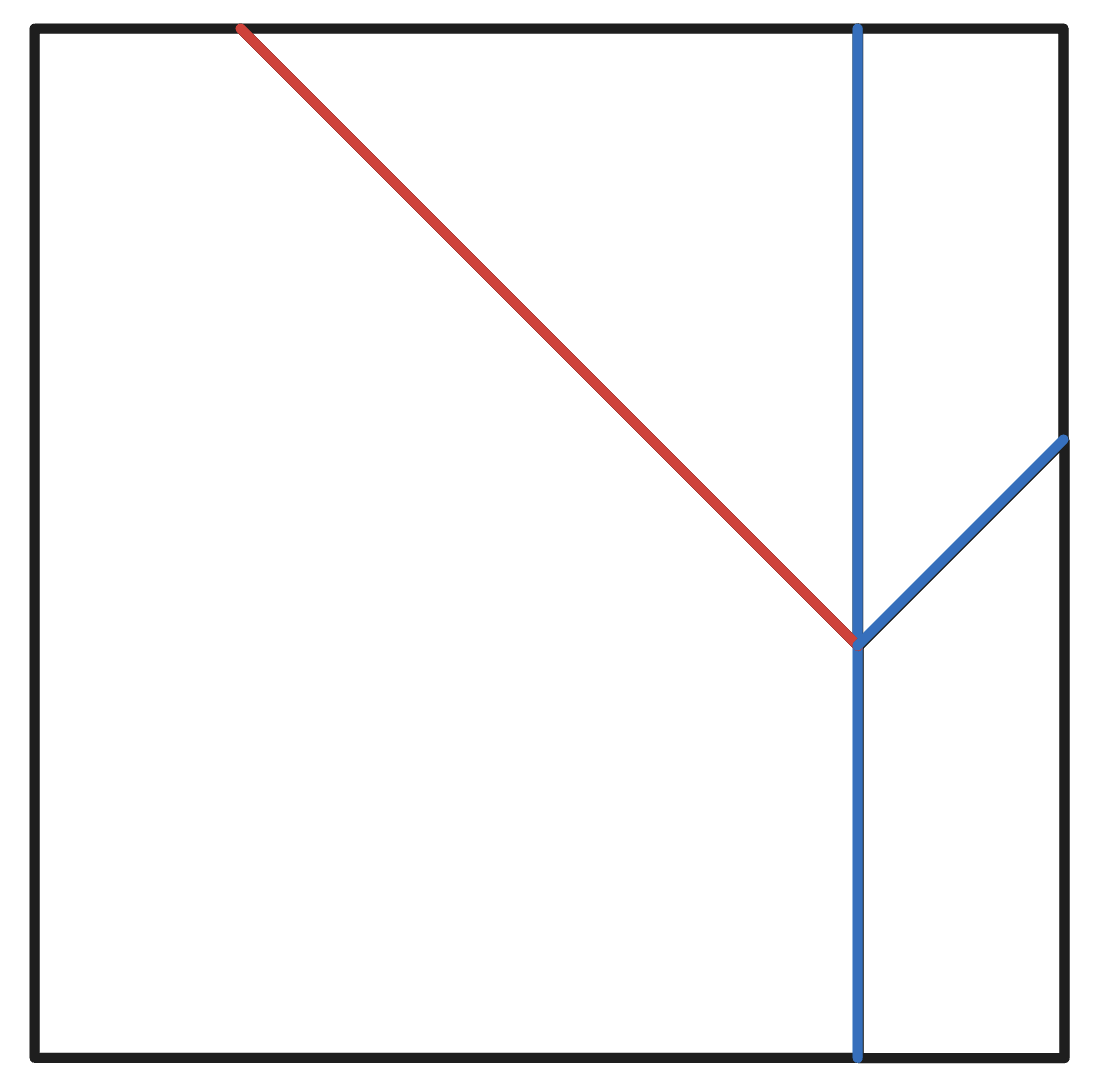
\includegraphics[width=0.4\textwidth]{assets/demo_creasepattern.png}
\caption{Example crease pattern that we want to determine the flat foldability of.}
\label{fig:demo_creasepattern}
\end{figure}

Let's say we get the crease pattern in Figure~\ref{fig:demo_creasepattern} and want to figure out - in a very hands on way - if this crease pattern is flat foldable.

To get a grasp of what a flatfolded configuration of the crease pattern might look like we can try to work out the general positioning of the faces relative to each other.

What I mean by that is that we use the face that a flat folded state will not introduce any new creases so we know every
uncreased area of the crease pattern will be a continious uncreased area in a flat folded configuration.

We also know about the creases that the paper here makes a 180 degree turn (ignoring any thickness of the paper) as any
other angle would elevate the folded structure into the 3rd dimension thus making it not a flat fold.

We can choose an arbitrary face as defining the frame of reference.
In this stage we're only interested in the relative position of the faces in the 2d plane in which the crease pattern is embedded.
To not get bogged down by the ordering of overlapping faces, let's free ourselves from the constraint that the paper is one continious / strongly connected object and only work with the shape of the faces for now.
Practically we might cut out each face. To not lose the crease information let's label the edges of each
face which connects to another face by what type of crease (M/V) it was and the id of the other face.

\begin{figure}[h]
\centering
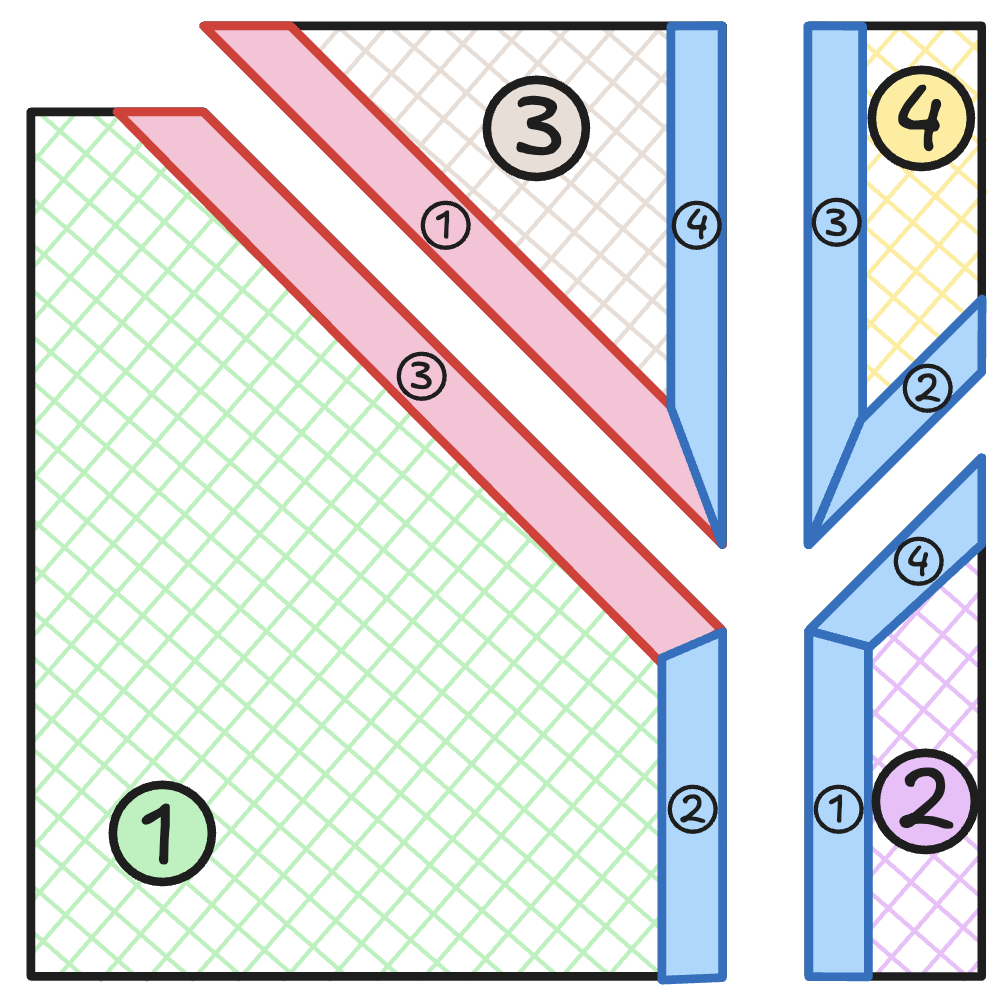
\includegraphics[width=0.4\textwidth]{assets/demo_faces.png}
\caption{Cut out faces of the crease pattern with face enumeration and edge labeling}
\label{fig:demo_faces}
\end{figure}

Continuing with the exemplary crease pattern from Figure~\ref{fig:demo_creasepattern} this step looks like Figure~\ref{fig:demo_faces}.

We have seperated the different faces of the crease pattern and assigned them ids from 1 to 4.
Each edge that was part of a crease is colored according to the crease type (red = mountain; blue = valley) while noting down the originally neighbouring face.

Let's use face 1 as the frame of reference.
As face 1 borders face 2 at a valley crease we know that any flat folded configuration will feature face 2 mirrored along the edge overlapping face 1.

\begin{figure}[h]
\centering
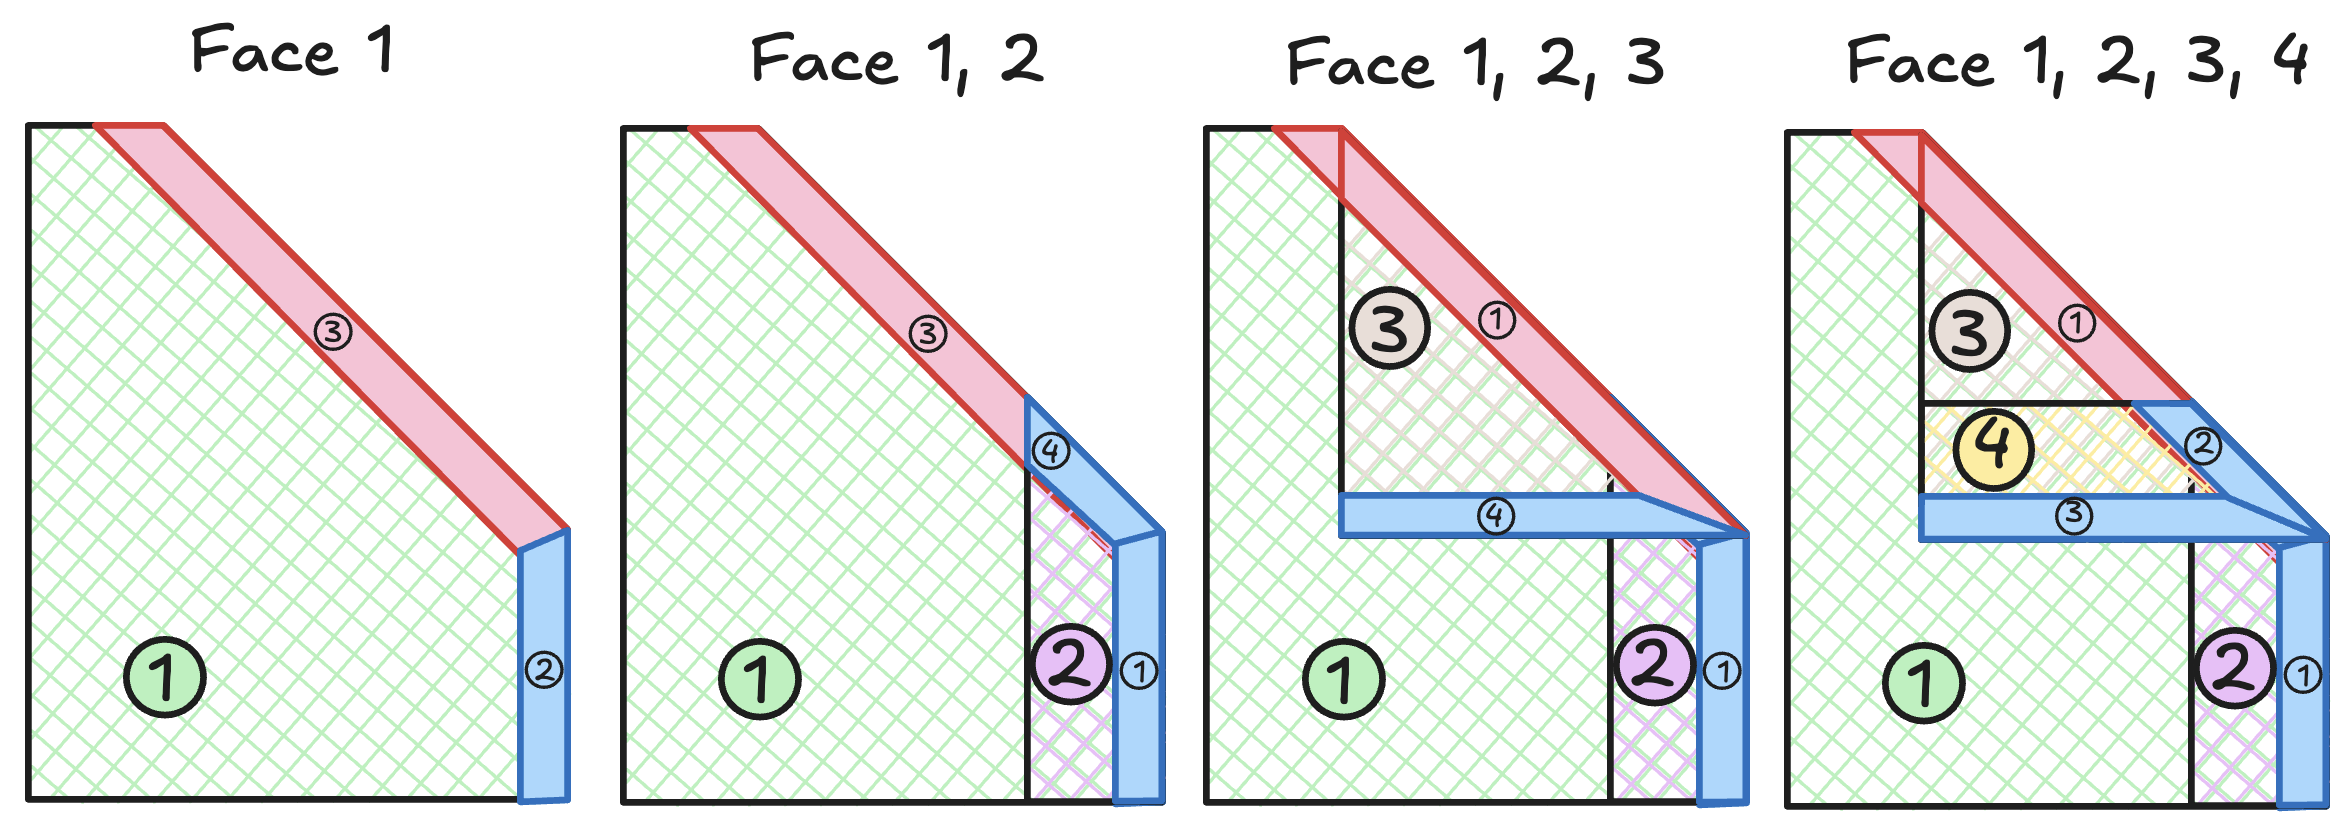
\includegraphics[width=\textwidth]{assets/demo_localflatfold.png}
\caption{Cut out faces of the crease pattern with face enumeration and edge labeling}
\label{fig:demo_localflatfold}
\end{figure}

By processing the faces in a neighbourly fashion (BFS / DFS / any other graph search on the face adjacency graph)
we know for certain where the next face will be located in the 2d plane.
This iterative construction is displayed step by step in Figure~\ref{fig:demo_localflatfold}.

In Figure~\ref{fig:demo_localflatfold} we can see this construction in 4 steps.

First we choose the face that defines the frame of reference and place it on the 2d plane.

Then we add face 2 which is neighbouring face 1. As they share the mountain valley to the right of face 1, the left edge
of face 2 aligns with this edge while the rest of face 2 extends to the left in order to fulfill the 180 degree that crease requires.

In the third step we position face 3 mirrored along the common edge with face 1.

Finally we position face 4 along the common edge with face 3.
As face 3 is already mirrored face 4 will be doubly mirrored aka not mirrored.

We could have used the common edge of face 4 with face 2 to find its relative positioning as well.
If a flat-folded configuration exists at all, these two constructions must agree; this is consistent with Kawasaki's
theorem at a single vertex, which states that for any node in a flat-foldable crease pattern when alternatively adding and subracting the angles of subsequent folds around the node the sum must equal to $0$. %% https://en.wikipedia.org/wiki/Kawasaki\%27s_theorem

If during this process we position a face so that not all of its edges align with the corresponding edges of neighboring
faces, then we can already conclude that the crease pattern is not flat-foldable.

Up to this point, our construction process has determined where each face is positioned in the 2D plane relative to our reference frame.
However, we don't have any guarantee that the reconnected paper will be intersection-free.
The faces we've positioned might be ordered in problematic ways when we consider them as parts of a continuous sheet of paper so that they intersect at their edges.

To address this, we need to introduce a third dimension back into our model - specifically, the stacking order of the faces. While the paper itself remains flat (zero thickness), we need to determine which face lies "above" or "below" another at any point where they overlap in our 2D projection.

The key insight is that we need to find a valid ordering of all faces such that:
1. Faces that share a crease are adjacent in the stacking order (no other face lies between them)
2. The relative orientation of adjacent faces respects the crease assignment (mountain or valley)
3. No face penetrates through a crease formed by two other faces

Rather than being constrained to the ordering that emerged from our construction steps, we should consider all possible orderings of the faces and check which ones satisfy these constraints.

This is where we can introduce the constraint of edge types more formally. At every point where creases intersect in our 2D projection, we need to examine the cross-sectional view to ensure the crease assignments are respected and no intersections occur.

Finally, we can categorize the types of violations that can occur in these cross-sections, leading us to the "taco" and "tortilla" classification that helps us systematically check for intersection-free configurations.

So now it's about reconnecting the faces that share common edges while respecting these ordering constraints.
As we've already determined the relative positioning of the faces, finding a flat folding is now reduced
to finding a ordering of the original faces such that the paper does not intersect itself.

The only way the paper can intersect itself is in the crossection of a crease.

Let's cheat a little and look at the crossectional view of the flat folded configuration.

\begin{figure}[h]
\centering
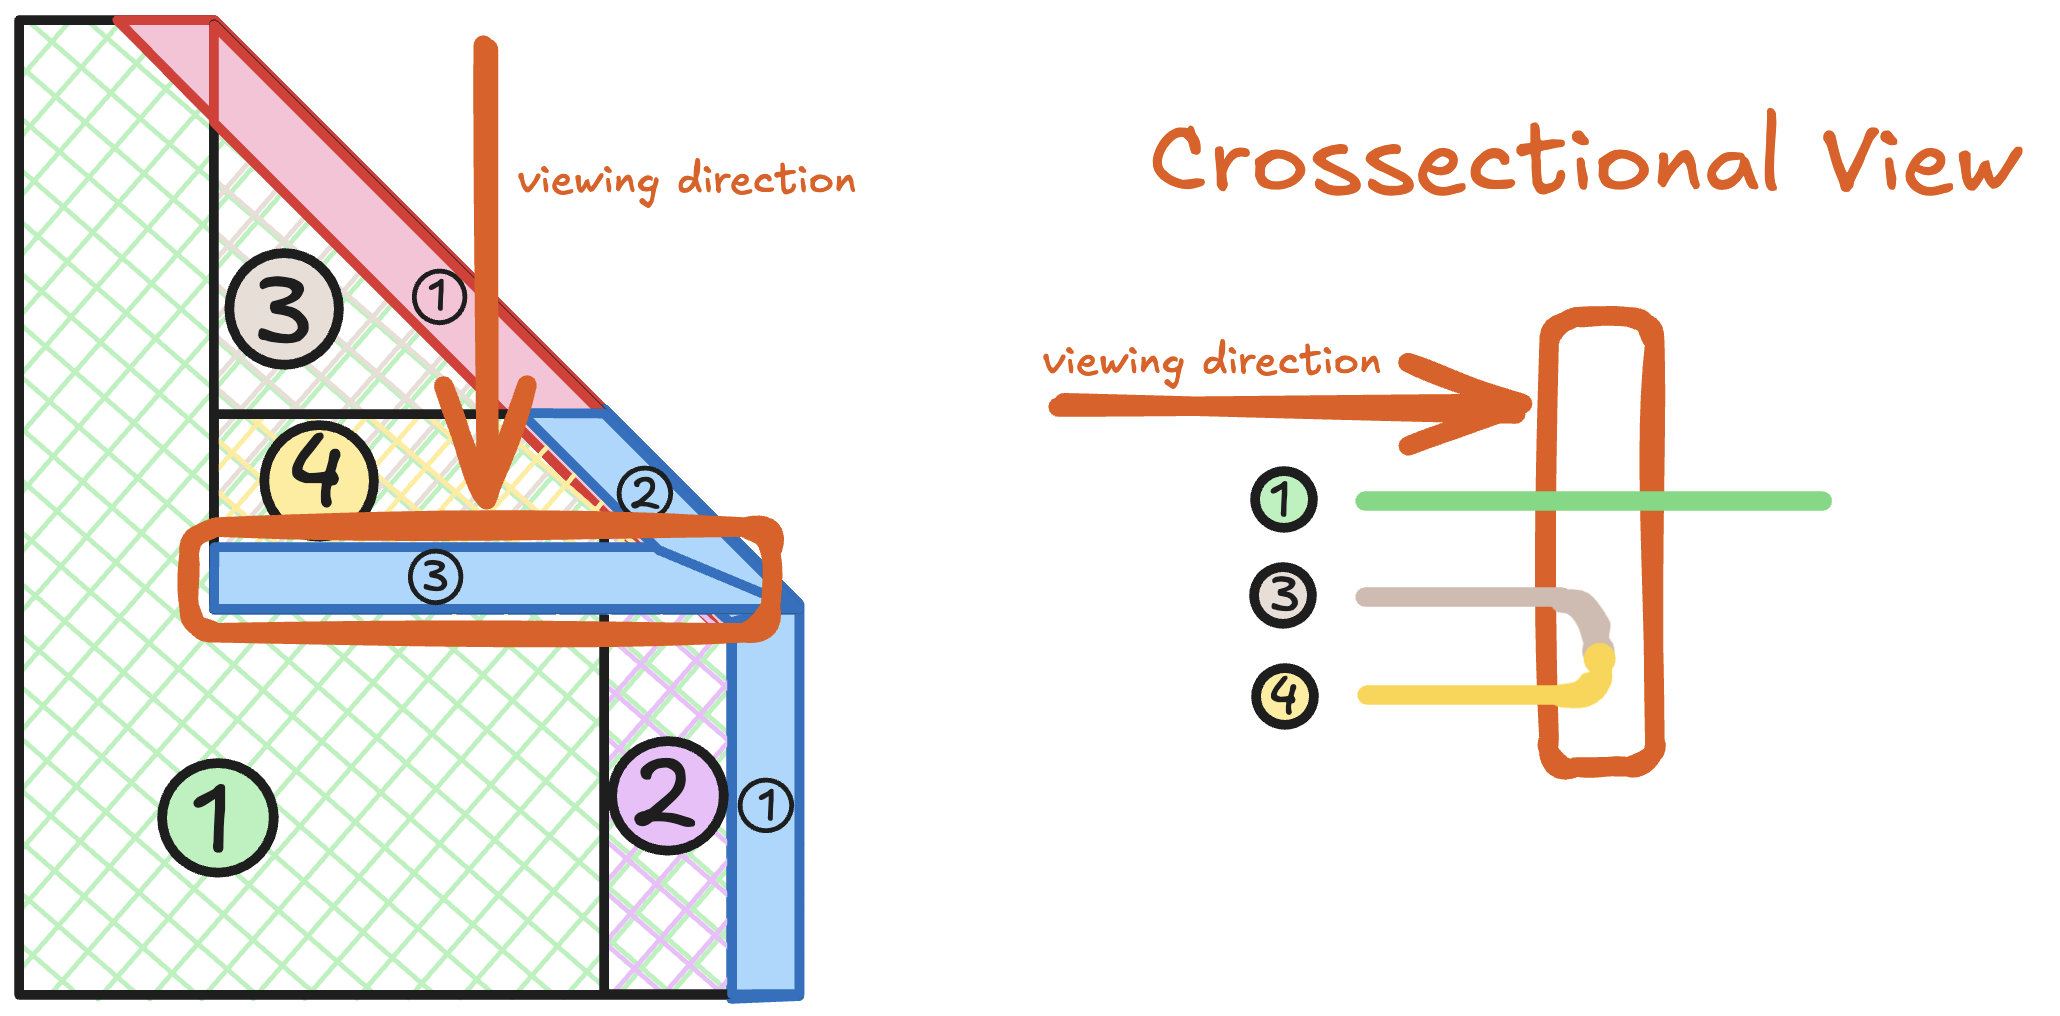
\includegraphics[width=0.6\textwidth]{assets/demo_csx_taco_tortilla.png}
\caption{Left: visual indication along which edge we look at the crossection of the system of faces; Right: Crossectional view along the highlighted edge; Face 1 is on top and penetrates the crossection, Face 4 is the bottom most face and forms a crease with Face 3 wich is layered in between Face 1 and 3.}
\label{fig:demo_csx_taco_tortilla}
\end{figure}

Looking at the crossection of the common edge of face 3 and 4 (see Figure~\ref{fig:demo_csx_taco_tortilla}) we see that face 1 penetrates the crossection while face 3 and 4 form a crease.
The crease between face 3 and 4 is a valley crease. Face 3 is mirrored while Face 4 is not.
Such we can confirm that this is a valid ordering of the faces (intersection free) and btw that any valid ordering must put face 3 above face 4.

\begin{figure}[h]
\centering
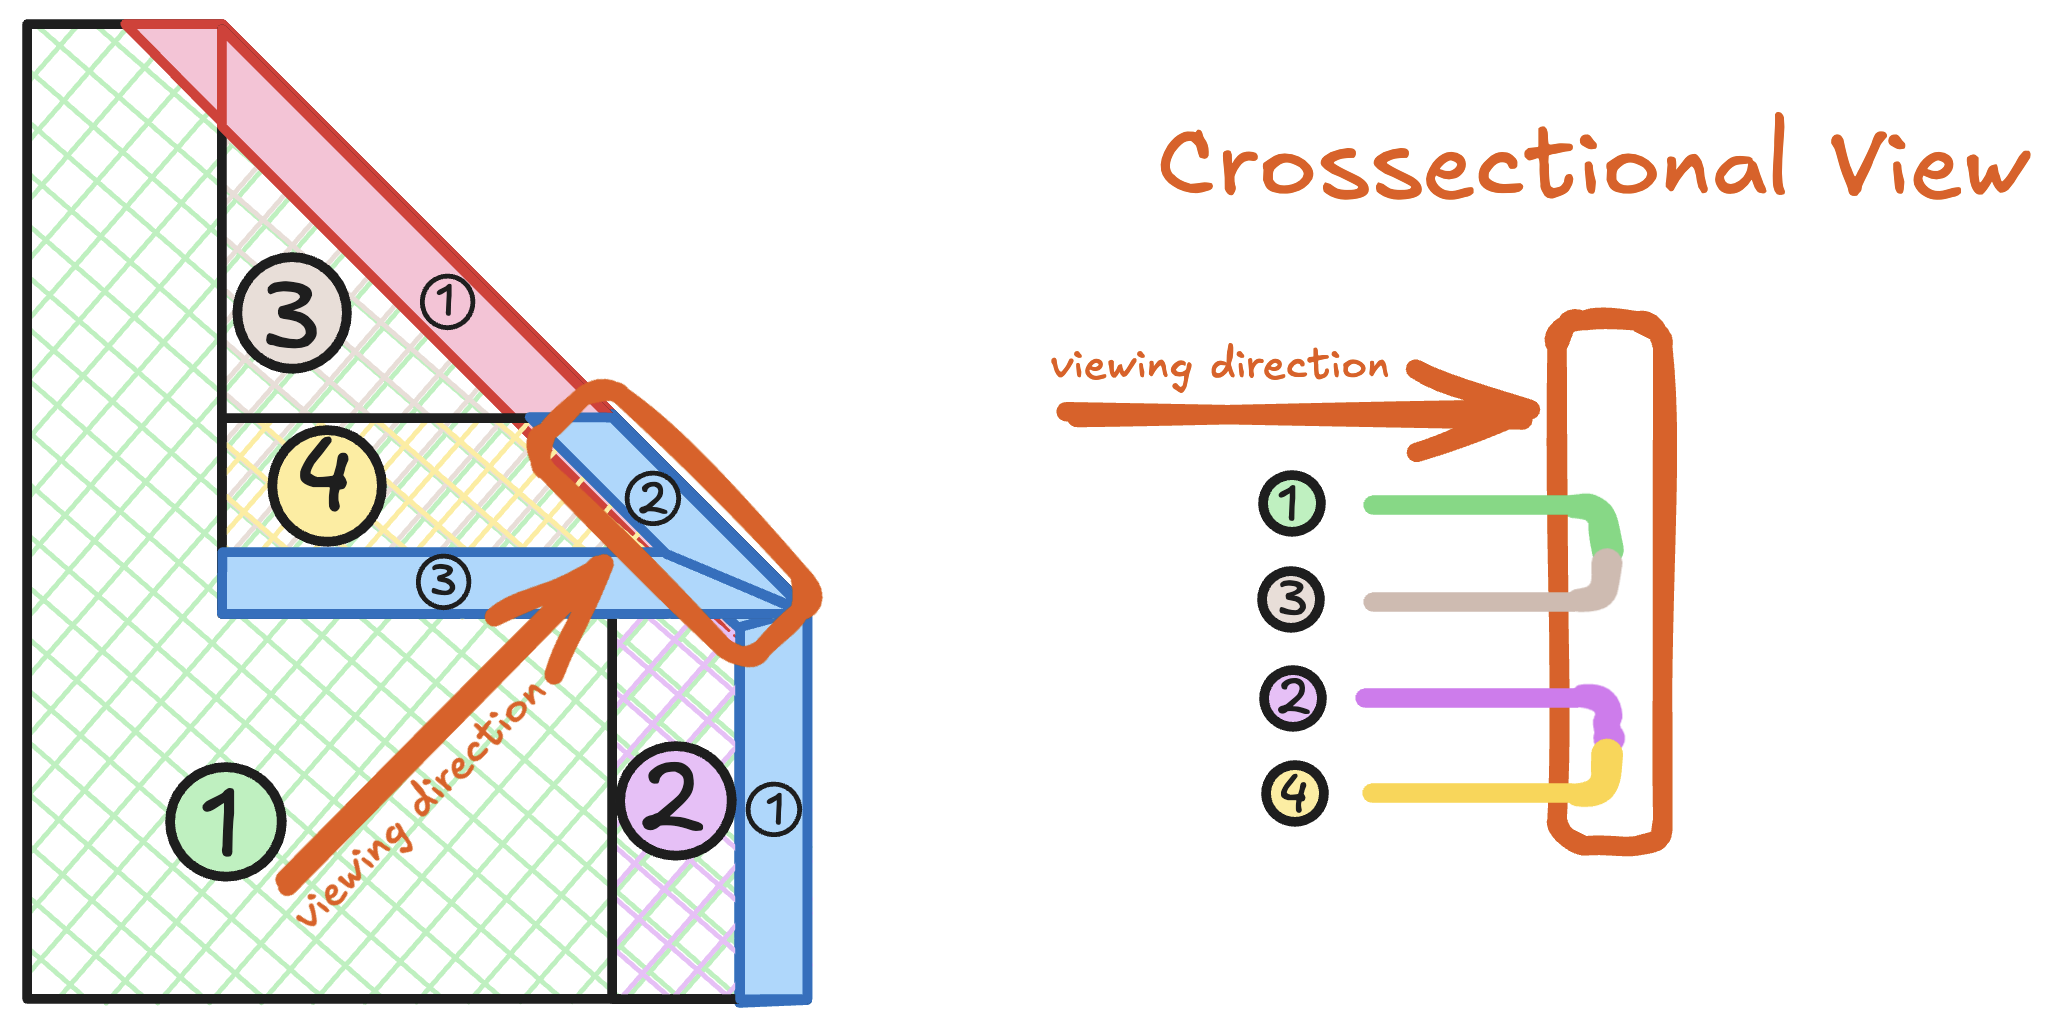
\includegraphics[width=0.6\textwidth]{assets/demo_csx_taco_taco.png}
\caption{Left: visual indication along which edge we look at the crossection of the system of faces; Right: Crossectional view along the highlighted edge; Face 1 and 3 are on top and connect to form a crease. Face 2 and 4 are below both and also connect to form a crease.}
\label{fig:demo_csx_taco_taco}
\end{figure}

Looking at the crossection of where both the crease between face 2 and 4 and part of the crease between the faces 1 and 3
land we can in the same way confirm that the crease assignment is obeyed as face 1 is above face 3 and face 2 is above face 4.

While making sure that the crease assignment is obeyed at all crossections is great we can use it to confirm the ordering is intersection free.

The two possible violations that can occur here can be categorized into 2 kinds.
As shown in the left in Figure~\ref{fig:demo_csx_bad_ordering} one kind of violation would be a face that penetrates a crease.
Here face 1 is between face 3 and face 4 but face 3 and 4 must form a crease in this crossection.

On the right side of Figure~\ref{fig:demo_csx_bad_ordering} you can see the other kind: two pairs of faces that form a crease in this cross section are interleaved.
This creates a self intersection of the paper.
 
\begin{figure}[h]
\centering
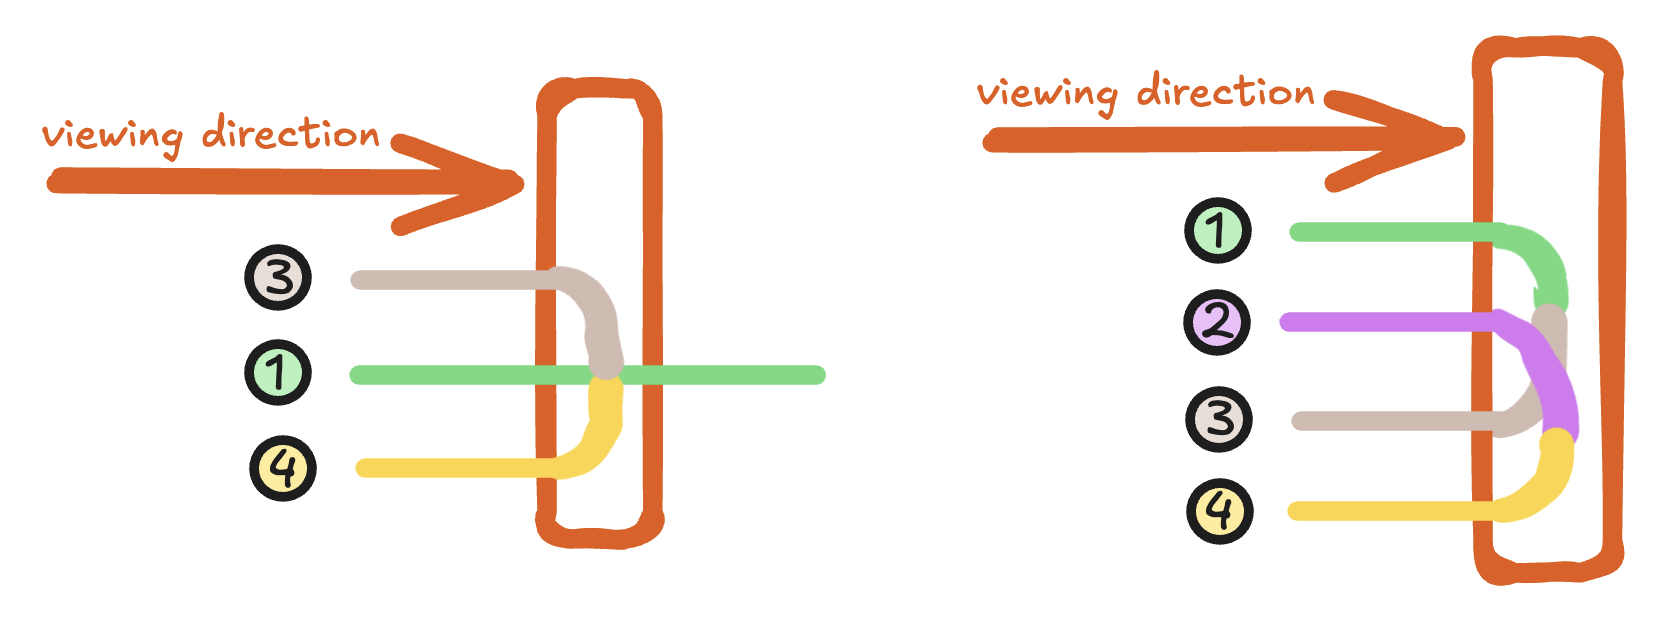
\includegraphics[width=0.6\textwidth]{assets/demo_csx_bad_ordering.png}
\caption{Alternate face orderings that create self intersections in the crossection examined in Figure~\ref{fig:demo_csx_taco_tortilla} (left) and in Figure~\ref{fig:demo_csx_taco_taco} (right).}.
\label{fig:demo_csx_bad_ordering}
\end{figure}

The two crossectional views above are chosen along an edge such that each plane either forms a crease at the crossection or penetrates the crossection along the total length.

We want to reduce the simplicity of this structure so that we 


\chapter{Formal Definitions}

Given the intuitive approach in the previous chapter I will formalize the algorithms and introduce
proper named states / steps.

\section{Crease Pattern}

There exist different formal definitions of crease patterns in literature.
The reference paper defines a crease pattern in a more general way that enables the study of crease patterns in arbitrary topologies with infinite numbers of creases.

To make the algorithm more accessible, we will use a more concrete definition of a crease pattern.
Thus we constrain ourselves to a planar geometric definition that captures the unfolded state of a crease pattern on flat paper with no cuts.

\begin{definition}[Crease Pattern]
~\\
A \textbf{Crease Pattern} is a tuple $C = (V, E, \phi, \alpha)$ with:
\begin{itemize}
    \item $V$ is a finite set of vertices
    \item $E \subseteq \binom{V}{2}$ is the set of undirected straight-line edges
    \item $\phi: V \hookrightarrow \mathbb{R}^2$ is an embedding mapping vertices to distinct points in the plane
    \item $\alpha: E \to \{\mathsf{M}, \mathsf{V}, \mathsf{B}\}$ assigns each edge a type: mountain ($\mathsf{M}$), valley ($\mathsf{V}$) or border ($\mathsf{B}$)
    \item All vertices $v \in V$ have degree $\delta(v) \geq 2$
    \item The geometric graph $(V, E, \phi)$ is connected and has no edge crossings
    \item The border edges $E_{\mathsf{B}} := \{e \in E \mid \alpha(e) = \mathsf{B}\}$ form a simple cycle
    \item All edges lie within or on the boundary of the polygon defined by the border edges $E_{\mathsf{B}}$
\end{itemize}
\end{definition}

%% maybe include a photo of a real world crease pattern and the representation of the crease pattern

\subsection{Faces}
Since $(V,E,\phi)$ is a connected planar graph embedded in $R^2$, it partitions the plane into a set of faces.
Let $F_C$ denote the set of bounded faces (excluding the outer infinite face).
For all faces $f \in F$, let $V_f \subseteq V$ denote the set of vertices on the boundary of $f$, and let $E_f \subseteq E$ denote the edges on the boundary of $f$.

\section{Local Flat Folding}

\begin{definition}[Local Flat Folding]
~\\
Let $C = (V, E, \phi, \alpha)$ be a crease pattern.\\
A function $\varphi: V \to \mathbb{R}^2$ is a \textbf{local flat folding} of $C$ if it satisfies:

\begin{enumerate}
    \item \textbf{Face preservation:} For each face $f \in F_C$, the point sets $\{\phi(v) \mid v \in V_f\}$ and $\{\varphi(v) \mid v \in V_f\}$ are congruent.
    % $\forall f \in F_C: \text{the point sets } \{\phi(v) \mid v \in V_f\} \text{ and } \{\varphi(v) \mid v \in V_f\} \text{ are congruent (same shape and size)}$
    \item \textbf{Reflection consistency:} For each crease edge $e = \{u,v\} \in E \setminus E_{\mathsf{B}}$ shared by faces $f_1, f_2 \in F_C$, the image of face $f_2$ under $\varphi$ is the reflection of the image of face $f_1$ across the line segment $\varphi(u)\varphi(v)$.
    % $\forall f_1, f_2 \in F_C \text{ with } E \ni \{v,w\} \in V_{f_1} \cap V_{f_2}:$ relative to $f_1$: $f_2$ is mirrored along their common edge.
\end{enumerate}
\end{definition}

\section{Shadow Graph / Master Graph}

The shadow graph is the Local Flat Folding graph but planarized / regularized, such that:

\begin{itemize}
    \item Vertecies that are mapped to the same point in the plane are merged
    \item Edges that intersect in a point are split at that point and a new vertex is inserted
    \item Edges that overlap are split and the overlapping part is merged together
    \item Edges retain the information about which crease(s) they represent
\end{itemize}

\section{Face Layering}

A order of the faces.


\section{Flat Foldability}

A face layering such that the paper does not self-intersect.

This is not rigid-foldability and there might not exist a sequence of folds which during each folding motion retains the rigidity of the faces but rather, that during a folding sequence it might be that the faces are deformed / bent.
An example of a crease pattern that is flat foldable but not rigid flat foldable can be seen in Figure \ref{fig:example_non_rigid}.
When folding the right side along the left valley crease onto the left side, the ``flaps'' of the right side must be bent to fit through the slit, to enable folding a second time along the right valley crease.
This is not a property of the concavety of the paper and crease patterns on a convex paper can be constructed such that faces must be bent during folding motions.

\begin{figure}[h]
\centering
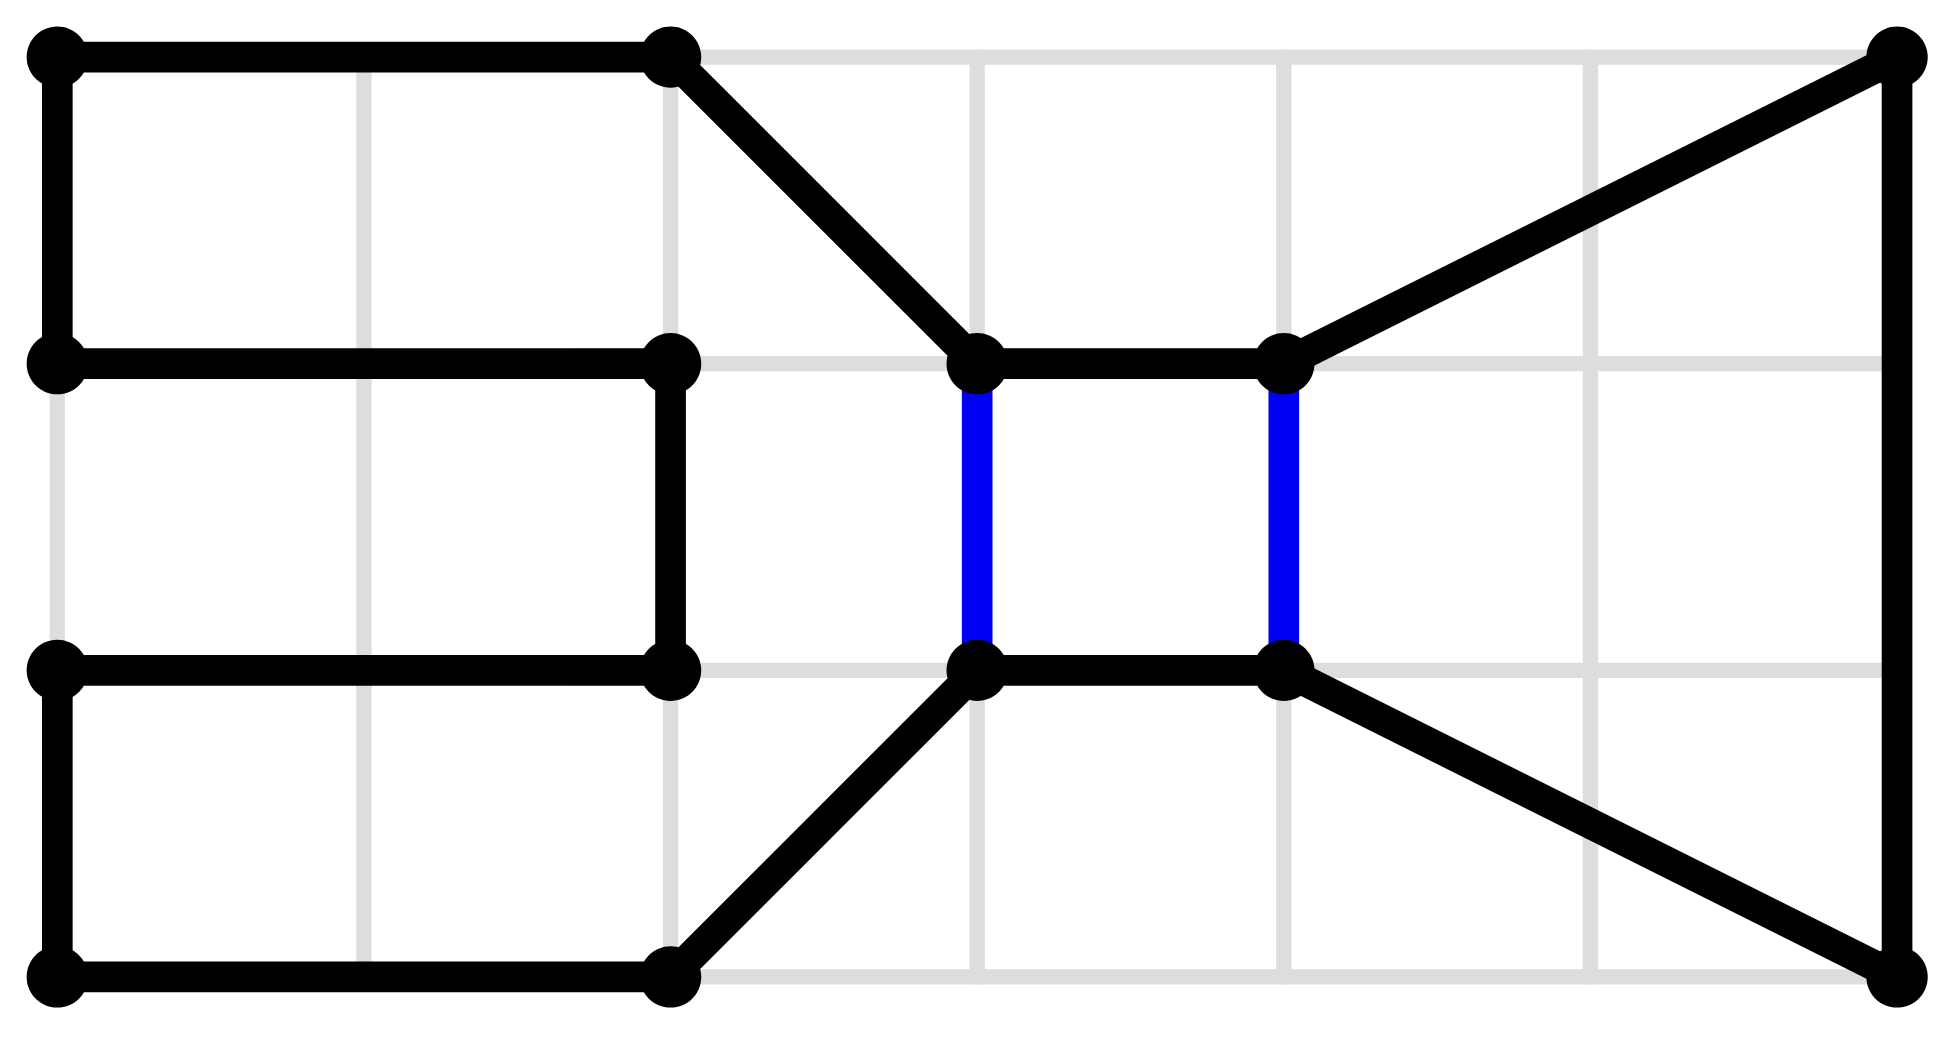
\includegraphics[width=0.6\textwidth]{assets/example_non_rigid.png}
\caption{Example of a crease pattern that is flat foldable but not rigid flat foldable.}.
\label{fig:example_non_rigid}
\end{figure}

An example of this is

\section{Cell-Adjacency Graph}

This is the dual graph of the shadow graph.

\section{Tractable: Tree-Width and Ply}

Tree-width is the tree-width of the cell-adjacency graph.
Ply is the maximum number of faces that overlap at any point in the plane.
This is the maximum number of faces a cell represents in the cell-adjacency graph.

When fixing tree-width and ply, the complexity of the algorithm is polynomial in the number of creases (edges) in the input and called ``tractable''.


\chapter{Algorithm}

\begin{lstlisting}
class NodeAttributes:
    position: tuple[float, float]

class EdgeAttributes:
    crease_type: Literal["M", "V", "B"]

class Graph:
    nodes: dict[int, NodeAttributes]
    edges: dict[tuple[int, int], EdgeAttributes]
\end{lstlisting}

\begin{lstlisting}
def bfs_iter(graph, start_node):
    queue = []
    visited = set()

    for start in graph.nodes():
        if start not in visited:
            queue.append(start)
            visited.add(start)
            while queue:
                node = queue.pop(0)
                yield node
                for neighbor in graph.neighbors(node):
                    if neighbor not in visited:
                        visited.add(neighbor)
                        queue.append(neighbor)
\end{lstlisting}




% A folded state of a crease pattern is a configuration of the paper in 3D space where:
% \begin{itemize}
%     \item we treat the paper as having zero thickness
%     \item The paper is folded along the creases according to their assigned types (mountain or valley) by 180 degrees
%     \item The paper does not self-intersect
%     \item the paper is continious and not cut or torn
%     \item the paper is not deformed in any way other than folding along the creases
%     \item The configuration is in 3D space but one dimension ist collapsed to the relative ordering of the layers
% \end{itemize}

% We can help visualize this by thinking of:
%  - the layers entirely parallel in a plane; this creates a set of parallel planes with $\epsilon$ distance between them
%  - at a crease the paper is folded by 180 degrees jumping from one plane to another one
%  - we replace the crease by a 90 degree turn in the paper in the third dimension, where extra paper length equal to $k \times \epsilon$ is added (when jumping $k$ layers "up" or "down")

% E.g. 


% A flat-folded state of a crease pattern $C = (V, E, \phi, \alpha)$ is a configuration where:
% \begin{enumerate}
% \item The paper lies entirely in a plane (the "folding plane")
% \item Each point in the folding plane may contain multiple layers of paper
% \item Layers have zero thickness but maintain a strict vertical ordering
% \item No self-intersection occurs between layers
% \item All creases are folded according to their assigned types
% \end{enumerate}

This does not capture that there's a way to fold the paper to a flat folded state without arbitrarily deforming the faces during the folding process.

%% TODO: <EXAMPLE>
